\documentclass[a4paper, 12pt]{article}
\usepackage{fancyhdr}
\usepackage{xcolor}
\usepackage{hyperref}
\usepackage{geometry}
\usepackage{tikz}
\usepackage{graphicx}
\usepackage{caption}
\usepackage{subcaption}
\usepackage{afterpage}
\usepackage{longtable}
\usepackage{booktabs}
\usepackage{background}
\usepackage{datetime}

\geometry{a4paper, margin=1in}

\definecolor{headerblue}{HTML}{00008B}
\definecolor{white}{HTML}{FFFFFF}
\definecolor{mylinkcolor}{HTML}{8b0000}
\definecolor{myurlcolor}{HTML}{8b0000}

% Background setup
\backgroundsetup{
  scale=1,
  color=black,
  opacity=1,
  angle=0,
  position=current page.south west,
  nodeanchor=south west,
  contents={%
    
\includegraphics[width=0.8in,height=\paperheight]{/var/www/html/alvo/flask/back/image_head.png}
  }
}

\pagestyle{fancy}
\fancyhf{}

% Header
\fancyhead[L]{
    \begin{tikzpicture}[remember picture, overlay]
        \fill[headerblue] (current page.north west) rectangle ([yshift=-1cm]current page.north east);
        \node[anchor=north west, inner sep=0pt, yshift=-1cm] at (current page.north west) {
\includegraphics[height=1cm]{/var/www/html/alvo/flask/back/image_head.png}}; % Adjusted height
    \end{tikzpicture}
}

% Footer
\fancyfoot[C]{
    
\begin{tikzpicture}[remember picture, overlay]
        \fill[headerblue] (current page.south west) rectangle ([yshift=1cm]current page.south east);
        \node[anchor=south, yshift=0.25cm] at (current page.south) {\color{white}\bfseries\thepage};
    \end{tikzpicture}
}

\renewcommand{\headrulewidth}{0pt}
\renewcommand{\footrulewidth}{0pt}

% Title and Date
\title{\Huge\textbf{\textcolor{headerblue}{Vulnerability Discovery Results}}}
\author{}
\date{\textcolor{headerblue}{\today} \\[0.5em] \textcolor{headerblue}{\currenttime} \\[0.5em] \textcolor{headerblue}{(UTC+2, PARIS)}}

% Adjust the style of sections (including \section*)
\usepackage{titlesec}
\titleformat{\section}[hang]{\Huge\bfseries\color{headerblue}}{}{0em}{}

% Hyperlink setup
\hypersetup{
    colorlinks=true,
    linkcolor=mylinkcolor,
    filecolor=magenta,
    urlcolor=myurlcolor,
}

\begin{document}
\maketitle
\thispagestyle{fancy}

\vspace{-1em}

\afterpage{\aftergroup\restoregeometry
    \thispagestyle{fancy}
    
    \begin{figure}[htbp]
        \centering
        
        \begin{subfigure}{\textwidth}
            \centering
            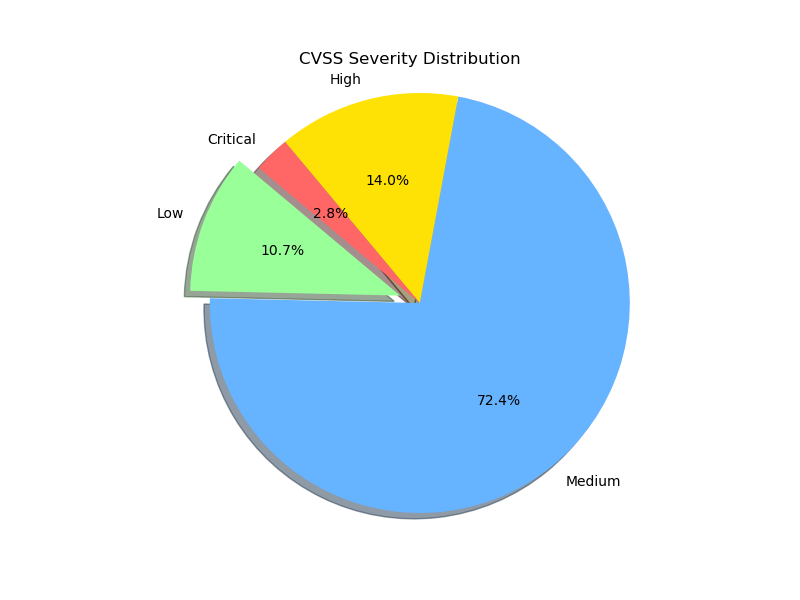
\includegraphics[width=0.9\linewidth]{/var/www/html/alvo/flask/back/alvo_pie_chart.png} % Adjust width of image as needed
            \caption{Figure 1: Pie Chart}
        \end{subfigure}
        
        \vspace{0.5cm}
        
        \begin{subfigure}{\textwidth}
            \centering
            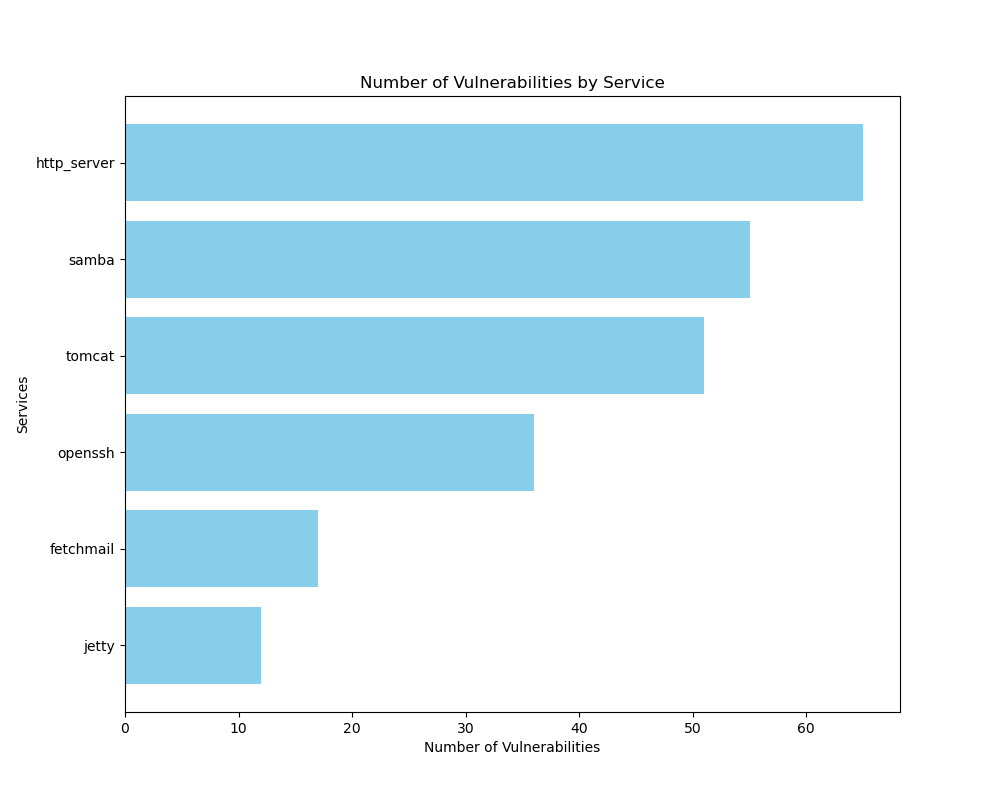
\includegraphics[width=0.9\linewidth]{/var/www/html/alvo/flask/back/alvo_bar_chart.png} % Adjust width of image as needed
            \caption{Figure 2: Bar Chart}
        \end{subfigure}
    \end{figure}
    \restoregeometry
}

$body$

\end{document}
